% 类氢原子的定态波函数
% 氢原子|波函数|束缚态|薛定谔方程

\pentry{玻尔原子模型\upref{BohrMd}, 球坐标和柱坐标中的定态薛定谔方程\upref{RadSE}} % 预备知识未完成

\textbf{类氢原子}被定义为原子核有 $Z$ 个质子(电荷为 $+Ze$, 有一个核外电子的原子/离子, 例如氢原子和失去一个电子的氦原子, 失去两个电子的锂离子. % 这个定义应该放在玻尔模型里面

类氢原子的定态薛定谔方程为
\begin{equation}\label{HWF_eq1}
-\frac{\hbar^2}{2m} \laplacian \psi(\bvec r) - \frac{Z}{r} \psi(\bvec r) = E \psi(\bvec r)
\end{equation}
类氢原子是唯一存在解析解的原子(离子).

我们这里只讨论束缚态, 即 $E < 0$ 的解.  从数学上, $E$ 取小于零的任意值时我们都能找到解, 但只有当 $E$ 取特定离散值的时候这些波函数才能归一化(否则没有物理意义). 由于类氢原子具有球对称性, 球坐标下的波函数具有最简单的形式. 波函数的表达式为
\begin{equation}\label{HWF_eq3}
\psi_{nlm} (r,\theta ,\phi) = R_{nl}(r) Y_{l,m}(\theta, \phi)
\end{equation}
其中 $n$ 是\textbf{主量子数}($n = 1, 2, \dots$), $l$ 是\textbf{角量子数}($l = 0, 1, \dots, n - 1$), $m$ 是\textbf{磁量子数}($m = -l, -l+1, \dots, l$). $R_{nl}(r)$ 是归一化的\textbf{径向波函数}, $Y_{l,m}(\theta, \phi)$ 是归一化的\textbf{球谐函数}(见“球谐函数列表\upref{YlmTab}”).

\begin{figure}[ht]
\centering
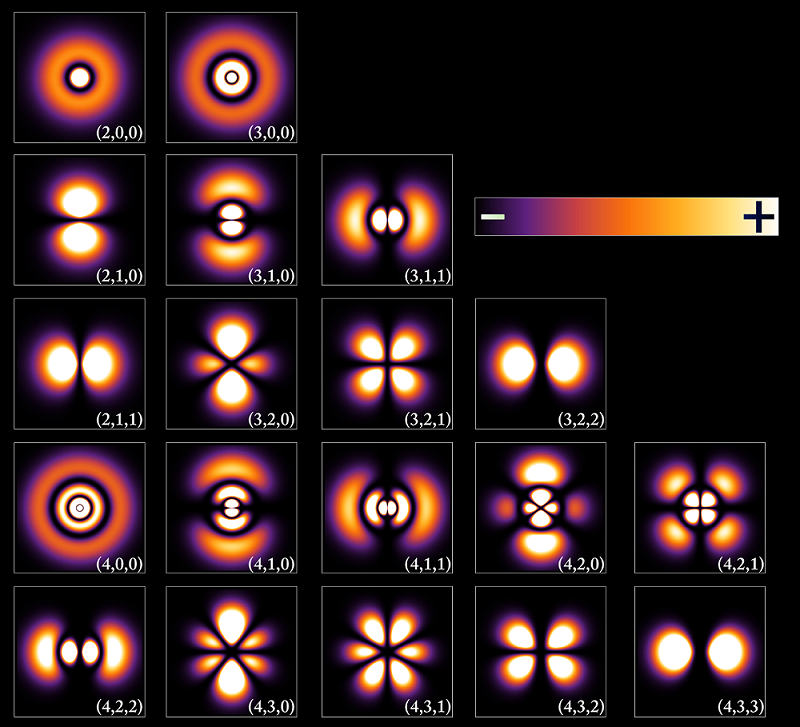
\includegraphics[width=13cm]{./figures/HWF_2.png}
\caption{氢原子波函数的概率密度 $\abs{\psi_{nlm}(\bvec r)}^2$ 的纵截面, 每个图中的三个数字分别是 $n, l, m$ 角量子数(来自维基百科)} \label{HWF_fig2}
\end{figure}

\subsubsection{径向波函数 $R_{nl}(r)$}

如果忽略原子核的运动, 以下的 $a$ 是玻尔半径, 如果不忽略, $a$ 就是约化玻尔半径.% 两个链接未完成
注意 $Z$ 和 $a$ 的作用是把径向波函数关于原点收缩 $Z/a$ 倍(并保持波函数归一化).
\begin{equation}\label{HWF_eq2}
R_{nl}(r) = \sqrt{\qty(\frac{2 Z}{na})^3 \frac{(n - l - 1)!}{2n (n + l)!}} \qty(\frac{2Zr}{na})^l  L_{n-l-1}^{2l+1}\qty(\frac{2Zr}{na}) \E^{-Zr/(na)}
\end{equation}
其中 $L_n^l(x)$ 是\textbf{连带拉盖尔多项式(associated Laguerre polynomial)}. 以下给出前几个径向以下给出前几个径向波函数, 注意所有径向波函数的值都是实数.

\begin{equation} % 已数值验证归一化和正交性
n = 1 \qquad
R_{10}(r) = 2\qty(\frac{Z}{a})^{3/2}\exp(-Zr/a)
\end{equation}
\begin{equation}
n = 2 \qquad
\leftgroup{
R_{20}(r) &= \frac{1}{\sqrt 2} \qty(\frac{Z}{a})^{3/2} \qty(1 - \frac12 \frac{Zr}{a}) \exp(-\frac{Zr}{2a})\\
R_{21}(r) &= \frac{1}{2\sqrt{6}} \qty(\frac{Z}{a})^{3/2} \frac{Zr}{a} \exp(-\frac{Zr}{2a})
}\end{equation}
\begin{equation}
n = 3 \qquad
\leftgroup{
R_{30}(r) &= \frac{2}{3\sqrt {3}} \qty(\frac{Z}{a})^{3/2} \qty(1 - \frac23 \frac{Zr}{a} + \frac{2}{27} \frac{Z^2r^2}{a^2}) \exp(-\frac{Zr}{3a})\\
R_{31}(r) &= \frac{8}{27\sqrt 6} \qty(\frac{Z}{a})^{3/2} \qty(1 - \frac16 \frac {Zr}{a}) \frac {Zr}{a} \exp(-\frac{Zr}{3a})\\
R_{32}(r) &= \frac{4}{81\sqrt {30}} \qty(\frac{Z}{a})^{3/2} \frac{Z^2r^2}{a^2} \exp(-\frac{Zr}{3a})}
\end{equation}
更多 $R_{n,l}$ 可以用 Mathematica 或者 Wolfram Alpha 生成, 如
\begin{lstlisting}[language=Mathematica]
n = 4; l = 1;
Sqrt[(2*Z/(n*a))^3 * Factorial[n-l-1]/(2*n*Factorial[n+l])]
*(2*Z*r/(n*a))^l*LaguerreL[n-l-1, 2l+1, 2Z*r/(n*a)] * Exp[-Z*r/(n*a)]
\end{lstlisting}

$Z = 1$ 时 $r R_{l,m}(r)$ 的\footnote{我们以后会看到 $r R_{l,m}(r)$ 比 $R_{l,m}(r)$ 更常用}\footnote{我们以后会看到 $r R_{l,m}(r)$ 比 $R_{l,m}(r)$ 更常用}函数图如\autoref{HWF_fig1}
\begin{figure}[ht]
\centering
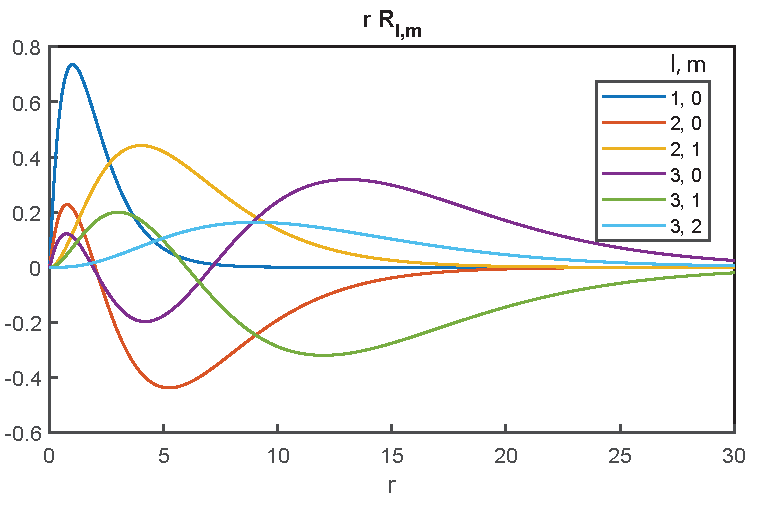
\includegraphics[width=12cm]{./figures/HWF_1.pdf}
\caption{径向波函数函数图} \label{HWF_fig1}
\end{figure}

\subsection{性质}
我们要求氢原子每个束缚态满足归一化条件
\begin{equation}
\int \abs{\Psi_{n,l,m}(\bvec r)} \dd[3]{r} = \int \int_0^\infty \abs{R_{n,l}(r) Y_{l,m}(\uvec r)}^2 r^2 \dd{r}\dd{\Omega} = 1
\end{equation}
先做角向积分, 球谐函数已经满足归一化条件% 链接未完成
\begin{equation}
\int \abs{Y_{l,m}(\uvec r)}^2 \dd{\Omega} = 1
\end{equation}
得到径向波函数的归一化条件为
\begin{equation}
\int [rR_{n,l}(r)]^2 \dd{r} = 1
\end{equation}

再来看正交性, 我们知道哈密顿算符的本征态之间两两正交(式中 $n',l',m'$ 至少有一个与 $n, l, m$ 不同)
\begin{equation}
\int \Psi_{n,l,m}^*(\bvec r) \Psi_{n',l',m'}(\bvec r) \dd[3]{r}
= \int \int_0^\infty R_{n,l}(r) R_{n',l'}(r) Y_{l,m}^*(\uvec r)  Y_{l',m'}(\uvec r) r^2 \dd{r}\dd{\Omega} = 0
\end{equation}
同样可以先对角向做积分, 若 $l',m'$ 至少有一个与 $l, m$ 不同, 那么积分直接为零, 径向波函数不需要任何正交条件(也的确不满足). 但若两个球谐函数相同, 即 $l' = l$, $m' = m$, $n' \ne n$, 那么角向积分等于 1, 径向波函数满足
\begin{equation}
\int \int_0^\infty R_{n,l}(r) R_{n',l}(r) r^2 \dd{r} = 0
\end{equation}

\subsection{径向概率分布}
我们来求径向概率分布 $P(r)$. $P(r)$ 的定义为: 发现粒子在 $r \in [a, b]$ (厚球壳)内的概率为 $\int_a^b P(r) \dd{r}$. 由于波函数的模长平方就是三维的概率密度, 有
\begin{equation}
\int_a^b P(r) \dd{r} = \int_a^b \int \abs{\frac1r \psi_{l,m}(r) Y_{l,m}(\uvec r)}^2 \dd{\Omega} r^2 \dd r
= \int_a^b \abs{\psi_{l,m}(r)}^2 \dd{r}
\end{equation}
对任意 $a, b > 0$ 都成立, 所以有
\begin{equation}
P(r) = \abs{\psi_{l,m}(r)}^2
\end{equation}

任意波函数可以表示为所有本征波函数的叠加
\begin{equation}
\Psi(\bvec r) = \frac1r \sum_{l,m} \psi_{l,m}(r) Y_{l,m}(\uvec r)
\end{equation}
其径向概率分布为
\begin{equation}\label{HWF_eq4}
\int_a^b P(r) \dd{r} = \int_a^b \int \abs{\frac1r \sum_{l,m}\psi_{l,m}(r) Y_{l,m}(\uvec r)}^2 \dd{\Omega} r^2 \dd r
= \sum_{l,m} \int_a^b \abs{\psi_{l,m}(r)}^2 \dd{r}
\end{equation}
对任意 $a, b > 0$ 都成立, 所以有
\begin{equation}
P(r) = \sum_{l,m} \abs{\psi_{l,m}(r)}^2
\end{equation}

\subsection{动量表象\ 动量分布}
要求动量表象下的波函数, 我们需要将位置表象的波函数投影到归一化的动量的本征矢上, 即三维傅里叶变换
\begin{equation}
\psi_{nlm}(\bvec p) = \braket{\bvec p}{\psi} = \frac{1}{\sqrt{2\pi}} \int \exp(-\I \bvec p \vdot \bvec r/\hbar) \psi(\bvec r) \dd[3]{r}
\end{equation}
这个积分在球坐标中完成才是最方便的, 具体方法我们将举例子说明(见\autoref{Pl2Ylm_ex1}\upref{Pl2Ylm}).

正如位置表象下位置的分布函数是 $\abs{\psi(\bvec r)}^2$, 动量表象下动量的分布函数是 $\abs{\psi(\bvec p)}^2$ (也符合测量理论).
